\documentclass[letterpaper, 11pt]{article} 

\usepackage{graphics,graphicx}
\usepackage{multicol} 
\usepackage{parskip}
\usepackage{amsmath}
\usepackage{multirow}
\usepackage[utf8]{inputenc}
\usepackage{fancyhdr}
\usepackage[title]{appendix}
\usepackage{wasysym}
\usepackage{url}
\usepackage{subcaption}

\usepackage[font=footnotesize,labelfont=small]{caption}
\captionsetup{width=0.85\linewidth}

\RequirePackage{geometry}
\geometry{margin=2cm}

\setlength{\parskip}{0.2cm}
\setlength{\parindent}{0pt}


\title{Project 4 Report: Signature-based Hit Predictor on AI Workloads}
\author{
Tai Duc Nguyen \\
ECEC 412: Modern Processor Design
}
\date{\today}

\begin{document}

\maketitle
\rule{\textwidth}{1pt}

\begin{abstract}
	Previously in project 3, different cache replacement policies: Least Recently Used (LRU) and Least Frequently Used (LFU) have been evaluated against AI Workloads. Continue that work, this project takes a look at the paper "SHiP: Signature-based Hit Predictor for High Performance Caching" by Wu et al. by evaluating their cache's architecture against the same 3 workloads as the last project.
\end{abstract}

\section{Introduction}
\label{intro}
	In order to achieve the objective of evaluating the performance of different cache replacement policies, a simulation was written in C by Shihao Song and Adarsha Balaji (available here: \url{https://github.com/Shihao-Song/Computer-Architecture-Teaching/tree/master/C621/Cache_Policy}). Using the framework established, a mechanism to test all pre-defined hardware configurations at once is written on top. After automating the testing of different configs, the LFU replacement policy is implemented in a similar fashion to the already existed code for the LRU replacement policy. And finally, the algorithm for SHiP cache predictor is written into the code for LRU and LFU.

\section{Simulation and Results}
	Using the same setup and simulation tool as Project 3, the algorithm for SHiP cache predictor is written on top. The pseudocode and its diagram is shown in Figure \ref{fig1} below.


	\begin{figure}[htb!]
		\centering
		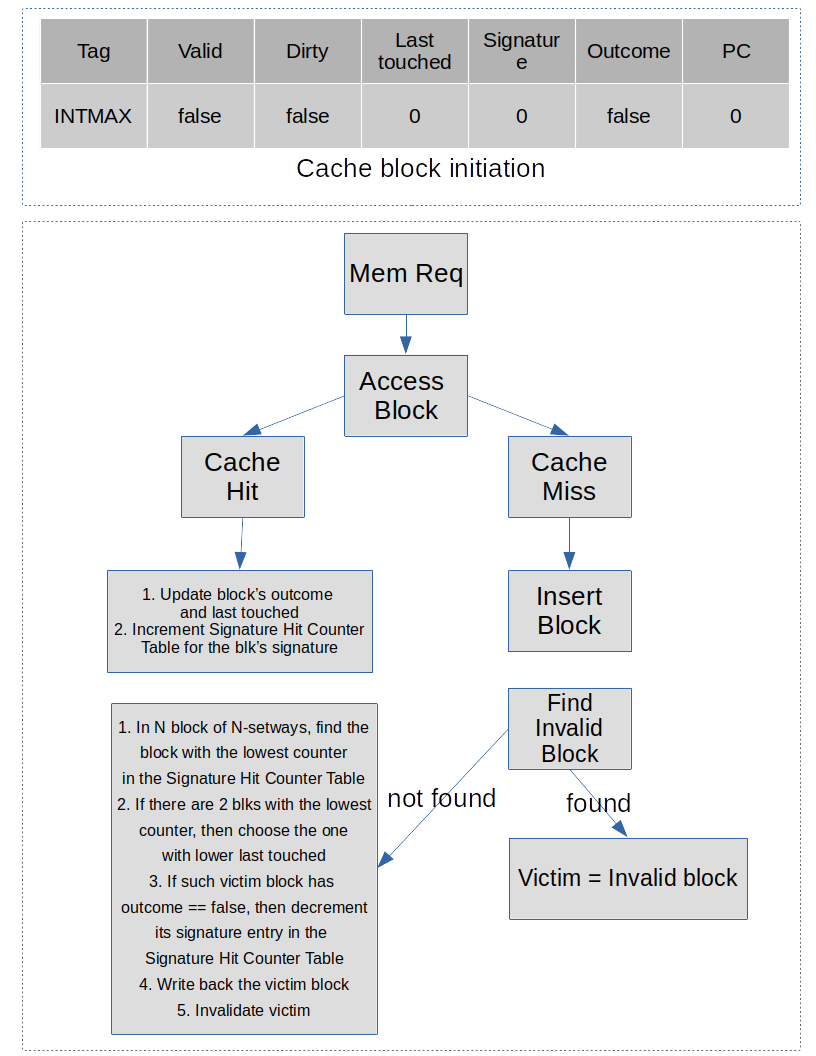
\includegraphics[width=0.7\linewidth]{pseudo_code_and_diagram.png}
		\caption{Sample output of the simulation}
		\label{fig1}
	\end{figure}

	\newpage
	
	Performing this simulation over all 3 memory traces (each trace includes many Load and Store instructions), the results are shown in graphs (Figure \ref{fig2a}, \ref{fig2b}, and \ref{fig2c}).
	
	\newpage
	
	\begin{figure}[htb!]
		\centering
		\begin{subfigure}[b]{.6\linewidth}
			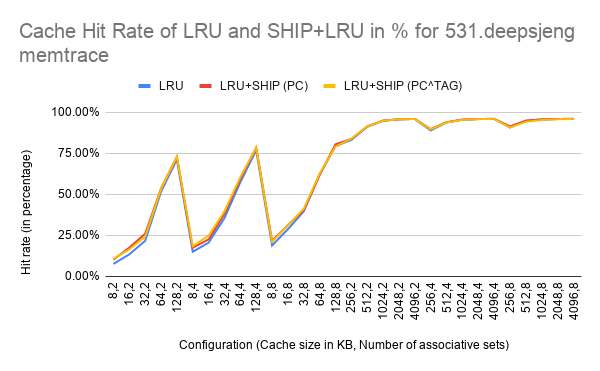
\includegraphics[width=\textwidth]{cache_hr_531_deepsjeng_memtrace.png}
			\caption{Results for 531.deepsjeng memory trace}
			\label{fig2a}
		\end{subfigure}
%		\hskip2em
		\begin{subfigure}[b]{.6\linewidth}
			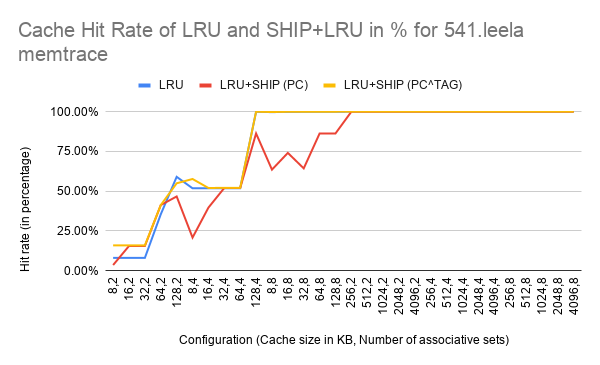
\includegraphics[width=\textwidth]{cache_hr_541_leela_memtrace.png}
			\caption{Results for 541.leela memory trace}
			\label{fig2b}
		\end{subfigure}
		\begin{subfigure}[b]{.6\linewidth}
			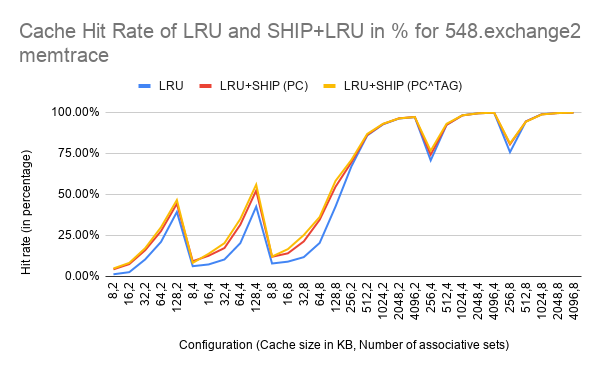
\includegraphics[width=\textwidth]{cache_hr_548_exchange2_memtrace.png}
			\caption{Results for 548.exchange2 memory trace}
			\label{fig2c}
		\end{subfigure}
		\caption{Simulation results. The x-axis have different hardware configurations with the first number being the cache size in KB and the second number being the number of associative sets. The y-axis is the cache hit rate in percentage.}
	\end{figure}

	\newpage
	
	
	To better see the differences in improvement of the SHiP cache predictor, Figure \ref{fig3a}, \ref{fig3b}, and \ref{fig3c} take the improvement ratios of SHiP+LRU using only the Program Counter (PC) to index the Signature Hit Counter Table (SHCT) over only LRU; and of SHiP+LRU using both PC and Memory Address over only using PC for SHCT indexing.
	
	\begin{figure}[htb!]
		\centering
		\begin{subfigure}[b]{.5\linewidth}
			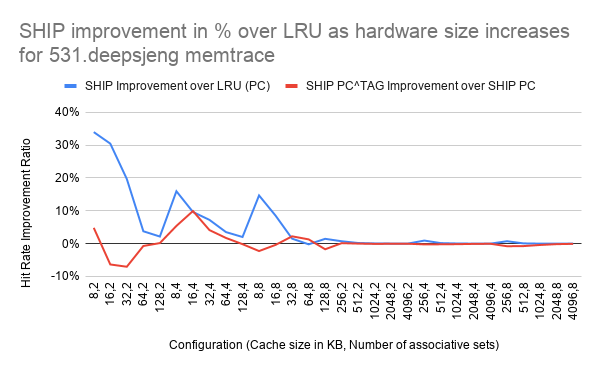
\includegraphics[width=\textwidth]{improvement_ratio_531_deepsjeng_memtrace.png}
			\caption{Improvement ratios for 531.deepsjeng memory trace}
			\label{fig3a}
		\end{subfigure}
		%		\hskip2em
		\begin{subfigure}[b]{.5\linewidth}
			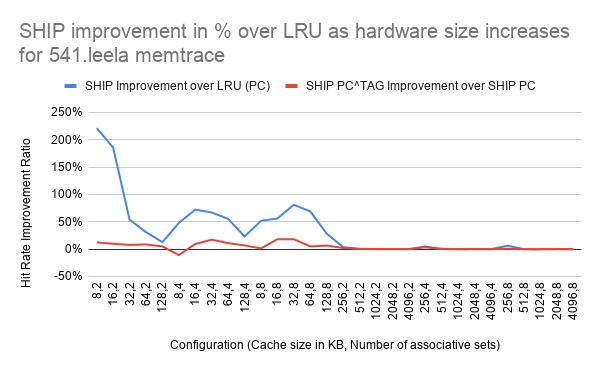
\includegraphics[width=\textwidth]{improvement_ratio_541_leela_memtrace.png}
			\caption{Improvement ratios for 541.leela memory trace}
			\label{fig3b}
		\end{subfigure}
		\begin{subfigure}[b]{.5\linewidth}
			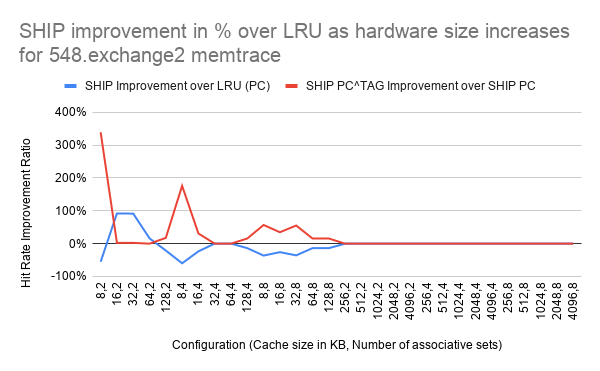
\includegraphics[width=\textwidth]{improvement_ratio_548_exchange2_memtrace.png}
			\caption{Improvement ratios for 548.exchange2 memory trace}
			\label{fig3c}
		\end{subfigure}
		\caption{Simulation results. The x-axis have different hardware configurations with the first number being the cache size in KB and the second number being the number of associative sets. The y-axis is the improvement ratio in percentage}
	\end{figure}
	
	From the 3 figures above, SHiP+LRU improves cache hit rate by a very large margin at low cache sizes (< 128KB) and low number of associative cache stores (< 4). However, when the cache size is greater than 128KB, with more than 2 associative cache sets, zero to very little improvement observed. In addition, the (PC XOR TAG) hashing algorithm in general does better than only using PC. This is probably due to the fact that the memtrace have many of instances where the same PC is requesting different memory locations.  
	
	The data for LFU is not shown in this experiment because it is determined from the last experiment that LFU does not provide a large cache hit rate improvement over LRU (best case: 4\%). The figures and data for LRU vs. LFU cache hit rate is shown in the Appendix Section.

\section{Discussion}
	SHiP cache prediction algorithm provides a way to better control the replacement of cache blocks, hence, allow useful blocks to retain in the cache more often and useless blocks to be removed from the cache more accurately. It is concluded from this experiment that: with the 3 AI Workloads tested, SHiP improves cache hit rate substantially when the cache size is smaller than 128KB or the number of associative cache stores is less than 4. At larger cache size or higher number of stores, SHiP increases the hit rate very slightly.
	
\section{Appendix}

	\begin{figure}[ht!]
	\centering
	\begin{subfigure}[b]{.48\linewidth}
		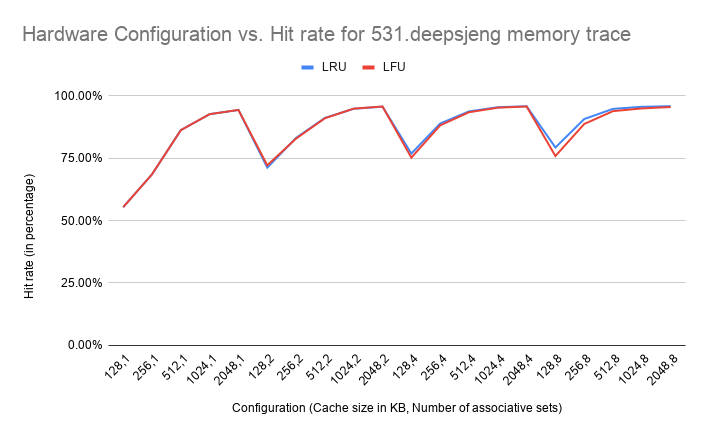
\includegraphics[width=\textwidth]{531_deepsjeng_results.png}
		\caption{Results for 531.deepsjeng memory trace}
		\label{fig2a}
	\end{subfigure}
	%		\hskip2em
	\begin{subfigure}[b]{.48\linewidth}
		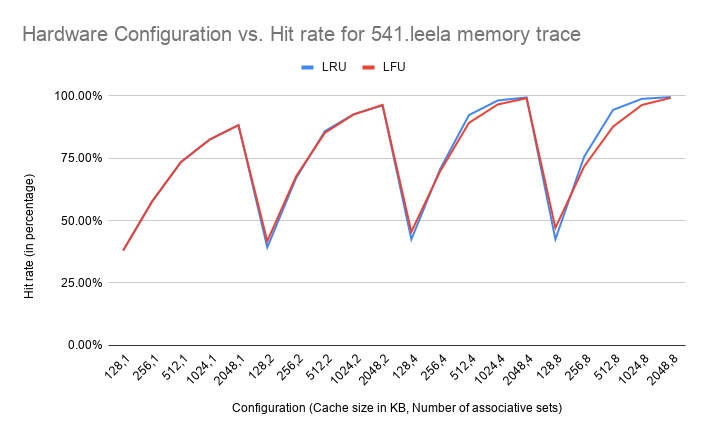
\includegraphics[width=\textwidth]{541_leela_results.png}
		\caption{Results for 541.leela memory trace}
		\label{fig2b}
	\end{subfigure}
	\begin{subfigure}[b]{.48\linewidth}
		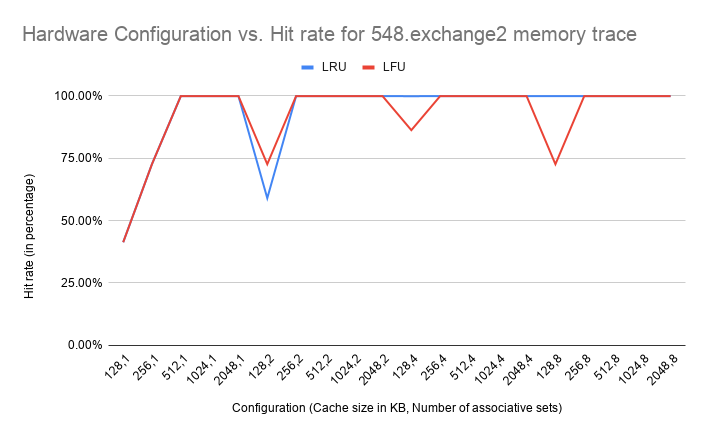
\includegraphics[width=\textwidth]{548_exchange2_results.png}
		\caption{Results for 548.exchange2 memory trace}
		\label{fig2c}
	\end{subfigure}
	%		\hskip2em
	\begin{subfigure}[b]{.48\linewidth}
		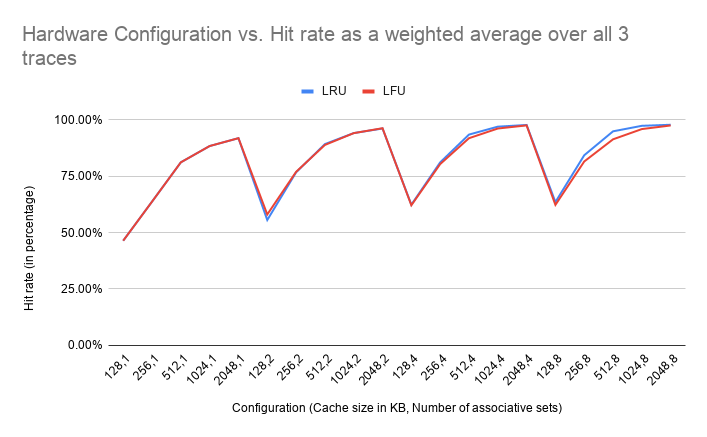
\includegraphics[width=\textwidth]{all_weighted_avg_results.png}
		\caption{Overall results as weighted averages of 3 traces}
		\label{fig2d}
	\end{subfigure}
	\caption{Simulation results for LRU vs. LFU. The x-axis have different hardware configurations with the first number being the cache size in KB and the second number being the number of associative sets. The y-axis is the cache hit rate in percentage.}
\end{figure}

\end{document}